%% LyX 2.4.4 created this file.  For more info, see https://www.lyx.org/.
%% Do not edit unless you really know what you are doing.
\documentclass[english,t]{beamer}
\usepackage{mathptmx}
\usepackage[T1]{fontenc}
\usepackage[latin9]{inputenc}
\usepackage{amssymb}
\usepackage{cancel}
\PassOptionsToPackage{normalem}{ulem}
\usepackage{ulem}

\makeatletter

%%%%%%%%%%%%%%%%%%%%%%%%%%%%%% LyX specific LaTeX commands.
%% Because html converters don't know tabularnewline
\providecommand{\tabularnewline}{\\}

%%%%%%%%%%%%%%%%%%%%%%%%%%%%%% Textclass specific LaTeX commands.
% this default might be overridden by plain title style
\newcommand\makebeamertitle{\frame{\maketitle}}%
% (ERT) argument for the TOC
\AtBeginDocument{%
  \let\origtableofcontents=\tableofcontents
  \def\tableofcontents{\@ifnextchar[{\origtableofcontents}{\gobbletableofcontents}}
  \def\gobbletableofcontents#1{\origtableofcontents}
}

%%%%%%%%%%%%%%%%%%%%%%%%%%%%%% User specified LaTeX commands.
\usetheme{Warsaw}
% or ...

\setbeamercovered{transparent}
% or whatever (possibly just delete it)
\setbeamercovered{invisible} %makes overlays invisible

%gets rid of navigation symbols
\setbeamertemplate{navigation symbols}{}

%\usepackage{hyperref}
%\usepackage[usenames,dvipsnames,table]{xcolor} %adds additional color options
\definecolor{links}{HTML}{2A1B81}
%\hypersetup{colorlinks,linkcolor=blue,urlcolor=links}

\usepackage{multicol}

\usepackage{tikz}
\usetikzlibrary{calc}
\usetikzlibrary{plotmarks}
\usepackage{pgfplots}
\pgfplotsset{compat=newest}

\usepackage{calc}
\usepackage[nomessages]{fp}

\usepackage{advdate}    % Advancing/saving dates
\usepackage{datetime}   % Dates formatting
\usepackage{datenumber} % Counters for dates
\usepackage[super]{nth}

\usepackage{etex}

\def\formatdateny{\csname noyear\languagename\expandafter\endcsname\formatdate}
\def\noyearenglish#1, \the\@year{#1}
\let\noyearamerican\noyearenglish
\let\noyearbritish\noyearenglish

%%%redefines column alignment to match vertically
%\define@key{beamerframe}{t}[true]{% top
  %\beamer@frametopskip=.2cm plus .5\paperheight\relax%
  %\beamer@framebottomskip=0pt plus 1fill\relax%
 % \beamer@frametopskipautobreak=\beamer@frametopskip\relax%
  %\beamer@framebottomskipautobreak=\beamer@framebottomskip\relax%
  %\def\beamer@initfirstlineunskip{}%
%}

%%provides pdf with 4 slides per page; don't forget to add 'handout' to remove overlays
%\usepackage{pgfpages}
%\pgfpagesuselayout{4 on 1}[a4paper, landscape, border shrink=7mm]
%\pgfpageslogicalpageoptions{1}{border code=\pgfusepath{stroke}}
%\pgfpageslogicalpageoptions{2}{border code=\pgfusepath{stroke}}
%\pgfpageslogicalpageoptions{3}{border code=\pgfusepath{stroke}}
%\pgfpageslogicalpageoptions{4}{border code=\pgfusepath{stroke}}
%%%Don't forget to add 'handout'

\makeatother

\usepackage{babel}
\begin{document}
\newcommand{\xmax}{2000}
\newcommand{\xmin}{0}
\newcommand{\xstep}{0} %must be xmin+n
\newcommand{\ymax}{500}
\newcommand{\ymin}{0}
\newcommand{\ystep}{0} %must be ymin+n

\newcounter{countEx} \setcounter{countEx}{0}
\newcounter{countProb} \setcounter{countProb}{0}
\resetcounteronoverlays{countEx} \resetcounteronoverlays{countProb}

\newcommand{\ex}[3]{
	\addtocounter{countEx}{1}
	\only<#1-#2>{\begin{exampleblock} {Example \chNum.\secNum.\arabic{countEx}.} #3	\end{exampleblock}}
}

\newcommand{\prob}[4]{
	\addtocounter{countProb}{1}
	\only<#1-#2>{\begin{exampleblock} {Problem  \chNum.\secNum.\arabic{countProb}.\,#3} #4	\end{exampleblock}}
}

\newcommand{\yline}[4]{
	(#2 - #4)/(#1 - #3)*(x - #1) + #2
}

\beamerdefaultoverlayspecification{<+->}

%%%%Chapter and Section numbers%%%%%
\newcommand{\chNum}{2}
\newcommand{\secNum}{1}
\newcommand{\secTitle}{Sets and Set Operations}

\title[Section \chNum.\secNum: \secTitle]{Section \chNum.\secNum: \secTitle}

\subtitle{Finite Mathematics~~MTH 107~~Fall 2014}

\author{Dr.\,James Ashe}

\titlegraphic{\includegraphics[height=2.75cm]{/home/jim/JamesAshe/MHU/images/MarsHilUniversityLogo-Virtical.png}}

\date{\formatdate{20}{8}{2014} and \formatdate{22}{8}{2014}}

\institute{Mars Hill University}

\makebeamertitle 
\begin{frame}{Chapter 2: Sets and Counting}

\begin{itemize}
\item [2.1] Sets and Set Operations
\item [2.2] Applications of Venn Diagrams
\item [2.3] Intro to Combinatorics
\item [2.4] Permutations \& Combinations
\end{itemize}
\end{frame}

\begin{frame}{Sets}

\vspace{-.75cm}
\begin{columns}


\column{5.5cm}
\begin{block}{Set}
 A \emph{set }is a well defined collection of distinct objects.

\begin{itemize}
\item Usually written as capital letters, e.g., \emph{A, B, C, }etc.
\end{itemize}
\end{block}
\footnotesize
\begin{itemize}
\item <2->[ex.] $\left\{ 0,2,4\right\} $
\item <3->[ex.] $R=\left\{ Billy,\,Bob,\,Bubba\right\} $
\item <4->[ex.] The set of letters in the alphabet

\begin{itemize}
\item <5->[]$\{a,b,c,\dots,x,y,z\}$
\end{itemize}
\item <6->[ex.] The set of positive integers.

\begin{itemize}
\item <7->[]$\left\{ 1,2,3,4,\dots\right\} $
\end{itemize}
\item <8->[ex.] The set of positive integers$<0$.

\begin{itemize}
\item <9->[]$\emptyset$ (the \emph{empty set}; $\emptyset\neq0$)
\end{itemize}
\end{itemize}

\column{5.5cm}
\begin{block}<11->{Element}
 The objects in the set are called \emph{elements} or \emph{members}.

\begin{itemize}
\item $x\in A$ means $x$ is an element in $A$.
\item $x\notin A$ means $x$ is not an element in $A$.
\end{itemize}
\end{block}
\footnotesize
\begin{itemize}
\item <12->[ex.] $2\in\left\{ 0,2,4\right\} $
\item <13->[ex.] $Carlton\notin R$
\item <14->[ex.] $h\in\{a,b,c,\dots,x,y,z\}$
\item <15->[ex.] $3.14\notin\left\{ 1,2,3,4,\dots\right\} $
\item <16->[ex.] $x\notin\emptyset$
\end{itemize}
\end{columns}
\end{frame}

\begin{frame}{Sets}

\vspace{-.75cm}
\begin{columns}


\column{4.5cm}
\begin{itemize}
\item <1->[]Two sets are \emph{equal} if they contain the same elements.

\begin{itemize}
\item <3->Order does not matter.
\item <5->We do not repeat elements
\end{itemize}
\item <7->[]A set can be given by,

\begin{itemize}
\item <8->[1.] description 
\item <10->[2.] \emph{tabular/roster }form
\item <12->[3.] \emph{set-builder} notation
\end{itemize}
\item <14->[]The \emph{cardinal number }of a set $A$ is the number of
elements in $A$.

\begin{itemize}
\item <15->Written, $n(A)$.
\end{itemize}
\end{itemize}

\column{6.5cm}

\footnotesize
\begin{itemize}
\item []
\item []
\item <2->[ex.]$\{0,2,4\}\neq\left\{ 0,2,4,1\right\} $
\item <4->[ex.]$\{0,2,4\}=\{2,4,0\}=\{4,0,2\}$
\item <6->[]Do not write $\{0,2,2,4\}$
\item []
\item []
\item <9->[ex.] The set of positive integers
\item <11->[ex.] $\{1,2,3,4,\dots\}$
\item <13->[ex.] $\left\{ x\mid x>0\mbox{ and }x\mbox{ is an integer}\right\} $
\item []
\item []
\item <16->[ex.] $n(\{0,2,4\})=3$
\item <17->[ex.] If $A=\{a,b\}$ then $n(A)=2$.
\end{itemize}
\end{columns}
\end{frame}

\begin{frame}{Sets}

\prob{1}{1}{Write the following set in \emph{tabular} and \emph{set-builder} form.}{The set of even, positive integers.}

\prob{2}{2}{Let $A=\{1,2,3,4\}$, $B=\{4,3,1,2\}$, and $C=\{1,2,3\}$}{True or False: $A=B$}

\prob{3}{3}{Let $A=\{1,2,3,4\}$, $B=\{4,3,1,2\}$, and $C=\{1,2,3\}$}{True or False: $4\notin A$}

\prob{4}{4}{Let $A=\{1,2,3,4\}$, $B=\{4,3,1,2\}$, and $C=\{1,2,3\}$}{Find $n(C)$}

\prob{5}{5}{Decide whether the following are \emph{true} or \emph{false}.}{$\{a,b,\dots,z\}=\{b,c,\dots,z\}$}

\prob{6}{6}{Let $\mathbb{Z}^{+}=\{1,2,\dots\}$ and  $\mathbb{N}=\{0,1,2,\dots\}$}{True or False: $\mathbb{Z}^{+} \neq \mathbb{N}$}

\prob{7}{7}{Let $\mathbb{Z}^{+}=\{1,2,\dots\}$ and  $\mathbb{N}=\{0,1,2,\dots\}$}{True or False: $n(\mathbb{Z}^{+}) = n(\mathbb{N})$}
\end{frame}

\begin{frame}{Subsets}

\vspace{-.75cm}
\begin{columns}


\column{6cm}
\begin{block}{Subset}
 a set $A$ is a \emph{subset} of a set $B$ if every element in
$A$ is also in $B$.

\begin{itemize}
\item []<2->$A\subseteq B$: $A$ is a subset of $B$
\item []<3->$A\nsubseteq B$: $A$ is \uline{not} a subset of $B$
\end{itemize}
\end{block}

\footnotesize
\begin{itemize}
\item <4->[ex.]

\begin{itemize}
\item <4->[]%
\begin{tabular}{l}
$A=\left\{ {\color{blue}3,4,5,6}\right\} $\tabularnewline
$B=\left\{ 2,{\color{blue}3,4,5,6}\mathpunct{\color{blue},}7,8\right\} $\tabularnewline
$C=\left\{ {\color{blue}3,4,5,6},9\right\} $\tabularnewline
\end{tabular}
\end{itemize}
\item <5-> $A\subseteq B$
\item <6->$C\nsubseteq B$
\item <7->$\emptyset\subseteq A$, $\emptyset\subseteq B$, and $\emptyset\subseteq C$
\item <8->$A\subseteq A$, $B\subseteq B$, $C\subseteq C$
\end{itemize}

\column{6cm }
\begin{itemize}
\item []\only<2->{%
\begin{minipage}[t]{0.33\textwidth}%
\begin{center}

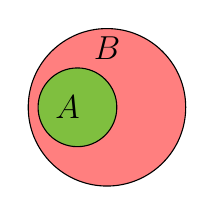
\begin{tikzpicture}     	\begin{scope}[scale=.5,shift={(3cm,-5cm)}, fill opacity=0.5,mytext/.style={text opacity=1,font=\large\bfseries}]         
		\draw[fill=red, draw = black] (0,0) circle (2);         
		\draw[fill=green, draw = black] (-0.75,0) circle (1);     
		\node[mytext] at (0,1.5) (B) {$B$};     		
		\node[mytext] at (-1,0) (A) {$A$};     	
	\end{scope}
\end{tikzpicture}
\\
\uncover<2->{$A\subseteq B$}
\par\end{center}%
\end{minipage}}\hspace{.5cm}\only<3->{%
\begin{minipage}[t]{0.33\textwidth}%
\begin{center}

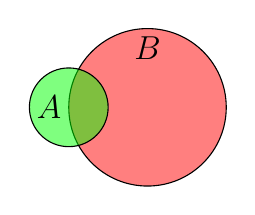
\begin{tikzpicture}     	\begin{scope}[scale=.5,shift={(3cm,-5cm)}, fill opacity=0.5,mytext/.style={text opacity=1,font=\large\bfseries}]         
		\draw[fill=red, draw = black] (0,0) circle (2);         
		\draw[fill=green, draw = black] (-2.0,0) circle (1);     
		\node[mytext] at (0,1.5) (A) {$B$};     		
		\node[mytext] at (-2.5,0) (B) {$A$};     	
	\end{scope}
\end{tikzpicture}
\\
\uncover<3->{$A\not\subseteq B$}
\par\end{center}%
\end{minipage}}
\item []
\item []
\item []\hspace{1cm} \only<4-7>{%
\begin{minipage}[t]{0.33\textwidth}%
\begin{center}

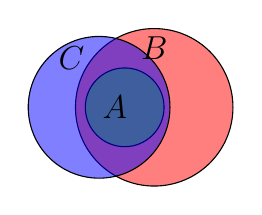
\begin{tikzpicture}     	\begin{scope}[scale=.5,shift={(3cm,-5cm)}, fill opacity=0.5,mytext/.style={text opacity=1,font=\large\bfseries}]         
		\draw[fill=red, draw = black] (0,0) circle (2);         
		\draw[fill=green, draw = black] (-0.75,0) circle (1);     
		\draw[fill=blue, draw = black] (-1.4,0) circle (1.8);

		\node[mytext] at (0,1.5) (B) {$B$};     		
		\node[mytext] at (-1,0) (A) {$A$};
		
		\node[mytext] at (-2.1,1.25) (C) {$C$};   	
	\end{scope}
\end{tikzpicture}
\\
\uncover<6->{$A\subseteq B$ and $C\not\subseteq B$}
\par\end{center}%
\end{minipage}}\only<8-8>{%
\begin{minipage}[t]{0.33\textwidth}%
\begin{center}

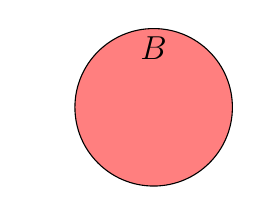
\begin{tikzpicture}     	\begin{scope}[scale=.5,shift={(3cm,-5cm)}, fill opacity=0.5,mytext/.style={text opacity=1,font=\large\bfseries}]         
		\draw[fill=red, draw = black] (0,0) circle (2);         
		\draw[fill=none, draw = none] (-0.75,0) circle (1);     
		\draw[fill=none, draw = none] (-1.4,0) circle (1.8);

		\node[mytext] at (0,1.5) (B) {$B$};     		
		%\node[mytext] at (-1,0) (A) {$A$};
		
		%\node[mytext] at (-2.1,1.25) (C) {$C$};   	
	\end{scope}
\end{tikzpicture}
\\
\uncover<8-8>{$B\subseteq B$}
\par\end{center}%
\end{minipage}}\only<9-9>{%
\begin{minipage}[t]{0.33\textwidth}%
\begin{center}

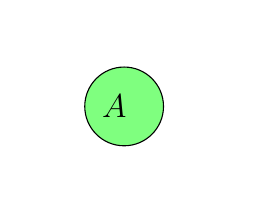
\begin{tikzpicture}     	\begin{scope}[scale=.5,shift={(3cm,-5cm)}, fill opacity=0.5,mytext/.style={text opacity=1,font=\large\bfseries}]         
		\draw[fill=none, draw = none] (0,0) circle (2);         
		\draw[fill=green, draw = black] (-0.75,0) circle (1);     
		\draw[fill=none, draw = none] (-1.4,0) circle (1.8);

		%\node[mytext] at (0,1.5) (B) {$B$};     		
		\node[mytext] at (-1,0) (A) {$A$};
		
		%\node[mytext] at (-2.1,1.25) (C) {$C$};   	
	\end{scope}
\end{tikzpicture}
\\
\uncover<9-9>{$A\subseteq A$}
\par\end{center}%
\end{minipage}}\only<10-10>{%
\begin{minipage}[t]{0.33\textwidth}%
\begin{center}

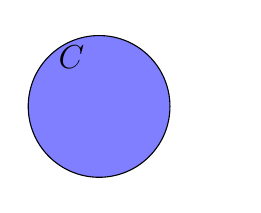
\begin{tikzpicture}     	\begin{scope}[scale=.5,shift={(3cm,-5cm)}, fill opacity=0.5,mytext/.style={text opacity=1,font=\large\bfseries}]         
		\draw[fill=none, draw = none] (0,0) circle (2);         
		\draw[fill=none, draw = none] (-0.75,0) circle (1);     
		\draw[fill=blue, draw = black] (-1.4,0) circle (1.8);

		%\node[mytext] at (0,1.5) (B) {$B$};     		
		%\node[mytext] at (-1,0) (A) {$A$};
		
		\node[mytext] at (-2.1,1.25) (C) {$C$};   	
	\end{scope}
\end{tikzpicture}
\\
\uncover<10-10>{$C\subseteq C$}
\par\end{center}%
\end{minipage}}
\end{itemize}
\end{columns}
\end{frame}

\begin{frame}{Subsets}

\begin{columns}


\column{5.5cm}
\begin{block}<1->{Proper Subset}
 a set $A$ is a \emph{proper subset} of a set $B$ if every element
in $A$ is also in $B$, and $A\neq B$.

\begin{itemize}
\item <2->[]$A\subset B$: $A$ is a proper subset of $B$.
\item []<3->$A\not\subset B$: $A\nsubseteq B$ and so $A$ is \uline{not}
a proper subset of $B$
\end{itemize}
\end{block}
\begin{itemize}
\item <3->[ex.]
\item <3->[]%
\begin{tabular}{l}
$A=\left\{ {\color{blue}3,4,5,6}\right\} $\tabularnewline
$B=\left\{ 2,{\color{blue}3,4,5,6}\mathpunct{\color{blue},}7,8\right\} $\tabularnewline
$C=\left\{ {\color{blue}3,4,5,6},9\right\} $\tabularnewline
\end{tabular}
\item <4->$A\subset B$ and $C\not\subset B$
\item <5->$B$ is not a proper subset $B$. 
\end{itemize}

\column{6cm }
\begin{itemize}
\item []\only<2->{%
\begin{minipage}[t]{0.33\textwidth}%
\begin{center}

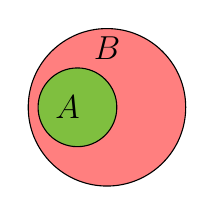
\begin{tikzpicture}     	\begin{scope}[scale=.5,shift={(3cm,-5cm)}, fill opacity=0.5,mytext/.style={text opacity=1,font=\large\bfseries}]         
		\draw[fill=red, draw = black] (0,0) circle (2);         
		\draw[fill=green, draw = black] (-0.75,0) circle (1);     
		\node[mytext] at (0,1.5) (B) {$B$};     		
		\node[mytext] at (-1,0) (A) {$A$};     	
	\end{scope}
\end{tikzpicture}
\\
\uncover<2->{$A\subset B$}
\par\end{center}%
\end{minipage}}\hspace{.5cm}\only<3->{%
\begin{minipage}[t]{0.33\textwidth}%
\begin{center}

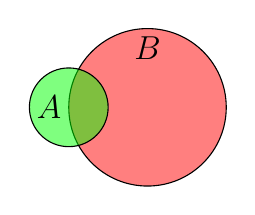
\begin{tikzpicture}     	\begin{scope}[scale=.5,shift={(3cm,-5cm)}, fill opacity=0.5,mytext/.style={text opacity=1,font=\large\bfseries}]         
		\draw[fill=red, draw = black] (0,0) circle (2);         
		\draw[fill=green, draw = black] (-2.0,0) circle (1);     
		\node[mytext] at (0,1.5) (A) {$B$};     		
		\node[mytext] at (-2.5,0) (B) {$A$};     	
	\end{scope}
\end{tikzpicture}
\\
\uncover<3->{$A\not\subset B$}
\par\end{center}%
\end{minipage}}
\item []
\item []
\item []\hspace{1cm} \only<3-5>{%
\begin{minipage}[t]{0.33\textwidth}%
\begin{center}

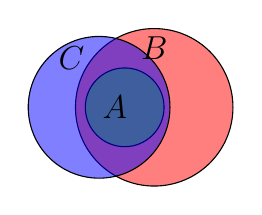
\begin{tikzpicture}     	\begin{scope}[scale=.5,shift={(3cm,-5cm)}, fill opacity=0.5,mytext/.style={text opacity=1,font=\large\bfseries}]         
		\draw[fill=red, draw = black] (0,0) circle (2);         
		\draw[fill=green, draw = black] (-0.75,0) circle (1);     
		\draw[fill=blue, draw = black] (-1.4,0) circle (1.8);

		\node[mytext] at (0,1.5) (B) {$B$};     		
		\node[mytext] at (-1,0) (A) {$A$};
		
		\node[mytext] at (-2.1,1.25) (C) {$C$};   	
	\end{scope}
\end{tikzpicture}
\\
\uncover<3-5>{$A\subseteq B$ and $C\not\subseteq B$}
\par\end{center}%
\end{minipage}}\only<6-6>{%
\begin{minipage}[t]{0.33\textwidth}%
\begin{center}

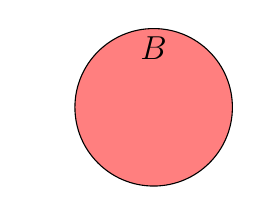
\begin{tikzpicture}     	\begin{scope}[scale=.5,shift={(3cm,-5cm)}, fill opacity=0.5,mytext/.style={text opacity=1,font=\large\bfseries}]         
		\draw[fill=red, draw = black] (0,0) circle (2);         
		\draw[fill=none, draw = none] (-0.75,0) circle (1);     
		\draw[fill=none, draw = none] (-1.4,0) circle (1.8);

		\node[mytext] at (0,1.5) (B) {$B$};     		
		%\node[mytext] at (-1,0) (A) {$A$};
		
		%\node[mytext] at (-2.1,1.25) (C) {$C$};   	
	\end{scope}
\end{tikzpicture}
\\
\uncover<6-6>{$B\not\subset B$ but $B\subseteq B$}
\par\end{center}%
\end{minipage}}
\end{itemize}
\end{columns}
\end{frame}

\begin{frame}{}

\vspace{-.5cm}

\center{\textbf{Venn Diagrams}}

\begin{figure}
\hfill%
\begin{minipage}[t]{0.33\textwidth}%
\begin{center}

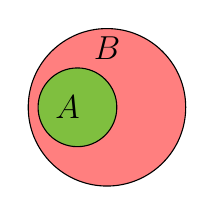
\begin{tikzpicture}     	\begin{scope}[scale=.5,shift={(3cm,-5cm)}, fill opacity=0.5,mytext/.style={text opacity=1,font=\large\bfseries}]         
		\draw[fill=red, draw = black] (0,0) circle (2);         
		\draw[fill=green, draw = black] (-0.75,0) circle (1);     
		\node[mytext] at (0,1.5) (B) {$B$};     		
		\node[mytext] at (-1,0) (A) {$A$};     	
	\end{scope}
\end{tikzpicture}
\\
\uncover<2->{$A\subseteq B$ and $A\subset B$}
\par\end{center}%
\end{minipage}\hfill%
\begin{minipage}[t]{0.33\textwidth}%
\begin{center}

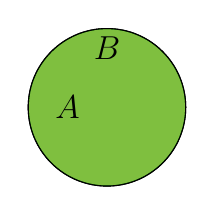
\begin{tikzpicture}     	\begin{scope}[scale=.5,shift={(3cm,-5cm)}, fill opacity=0.5,mytext/.style={text opacity=1,font=\large\bfseries}]         
		\draw[fill=red, draw = black] (0,0) circle (2);         
		\draw[fill=green, draw = black] (0.0,0) circle (2);     
		\node[mytext] at (0,1.5) (B) {$B$};     		
		\node[mytext] at (-1,0) (A) {$A$};     	
	\end{scope}
\end{tikzpicture}
\\
\uncover<3->{$A\subseteq B$}
\par\end{center}%
\end{minipage}\hfill%
\begin{minipage}[t]{0.33\textwidth}%
\begin{center}

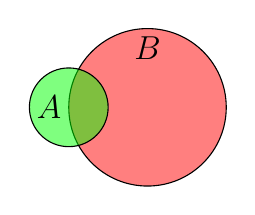
\begin{tikzpicture}     	\begin{scope}[scale=.5,shift={(3cm,-5cm)}, fill opacity=0.5,mytext/.style={text opacity=1,font=\large\bfseries}]         
		\draw[fill=red, draw = black] (0,0) circle (2);         
		\draw[fill=green, draw = black] (-2.0,0) circle (1);     
		\node[mytext] at (0,1.5) (A) {$B$};     		
		\node[mytext] at (-2.5,0) (B) {$A$};     	
	\end{scope}
\end{tikzpicture}
\\
\uncover<4->{$A\not\subset B$}
\par\end{center}%
\end{minipage}\hfill
\end{figure}

\prob{5}{5}{Let $A=\{2,4,6,10\}$, $B=\{2,4,8,10\}$, $C=\{4,8,12\}$, $D=\{2,10\}$, $E=\{6\}$, and $U=\{2,4,6,8,10,12,14\}$. Insert $\subseteq$ or $\nsubseteq$ to make the statement true.}{\center $A$\underline{\hspace{.5cm}}$E$}\prob{6}{6}{Let $A=\{2,4,6,10\}$, $B=\{2,4,8,10\}$, $C=\{4,8,12\}$, $D=\{2,10\}$, $E=\{6\}$, and $U=\{2,4,6,8,10,12,14\}$. Insert $\subseteq$ or $\nsubseteq$ to make the statement true.}{\center $\emptyset$\underline{\hspace{.5cm}}$A$}\prob{7}{7}{Let $A=\{2,4,6,10\}$, $B=\{2,4,8,10\}$, $C=\{4,8,12\}$, $D=\{2,10\}$, $E=\{6\}$, and $U=\{2,4,6,8,10,12,14\}$. Insert $\subseteq$ or $\nsubseteq$ to make the statement true.}{\center $A$\underline{\hspace{.5cm}}$U$}

\prob{8}{8}{Let $A=\{2,4,6,10\}$, $B=\{2,4,8,10\}$, $C=\{4,8,12\}$, $D=\{2,10\}$, $E=\{6\}$, and $U=\{2,4,6,8,10,12,14\}$. Insert $\subseteq$ or $\nsubseteq$ to make the statement true.}{\center $A$\underline{\hspace{.5cm}}$U$}
\end{frame}

\begin{frame}{Set Operations}

\begin{columns}


\column{6cm}

\vspace{-.75cm}
\begin{block}{Union}
The \emph{union }of $A$ and $B$ is the set of all elements in $A$
\uline{or} $B$

\begin{itemize}
\item $A\cup B=\left\{ x\mid x\in A\mbox{ or }x\in B\right\} $
\end{itemize}
\end{block}

\begin{block}<4->{Intersection}
The \emph{intersection }of $A$ and $B$ is the set of all elements
in $A$ \uline{and} $B$

\begin{itemize}
\item $A\cap B=\left\{ x\mid x\in A\mbox{ and }x\in B\right\} $
\end{itemize}
\end{block}

\begin{block}<9->{complement}
The \emph{complement }of $A$ is the set of everything in $U$ but
\uline{not} in $A$.

\begin{itemize}
\item $A'=\left\{ x\mid x\notin A\mbox{ and }x\in U\right\} $
\end{itemize}
\end{block}

\column{5.5cm}

%%%union%%%
\only<1-1>{%%%%A uncolored; B uncolored%%%%%
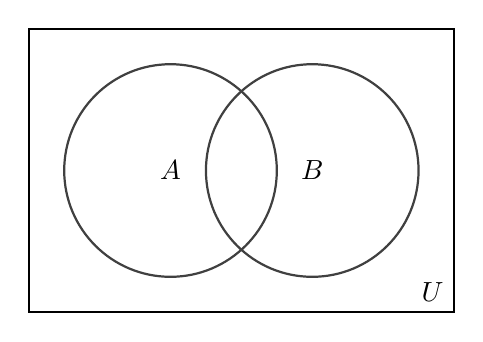
\begin{tikzpicture}[scale=.9]
	\def\circleA{(0,0) circle (1.5)} %A
	\def\circleB{(0:2) circle (1.5)} %B

	\colorlet{circle edgeA}{black!75} 
	\colorlet{circle areaA}{red!100}
	\colorlet{circle edgeB}{black!75} 
	\colorlet{circle areaB}{green!100}

	\tikzset{
		filledA/.style={fill=circle areaA, draw=circle edgeA, thick},
		filledB/.style={fill=circle areaB, draw=circle edgeB, thick},
		outlineA/.style={draw=circle edgeA, thick},
		outlineB/.style={draw=circle edgeB, thick},
	}

	\begin{scope}[fill opacity=0.5]         
			%\fill[filledB] \circleB;    
			%\fill[filledA] \circleA;
	\end{scope}

	\draw[outlineA] \circleA node {$A$}; 
	\draw[outlineB] \circleB node {$B$}; 
	%\node[anchor=south] at (current bounding box.north) {$A \cup B$}; 
	\draw[thick] (-2,-2) rectangle (4,2) node[anchor=south east] at (current bounding box.south east) {$U$}; 
\end{tikzpicture} }\only<2-2>{%%%%A colored; B uncolored%%%%%
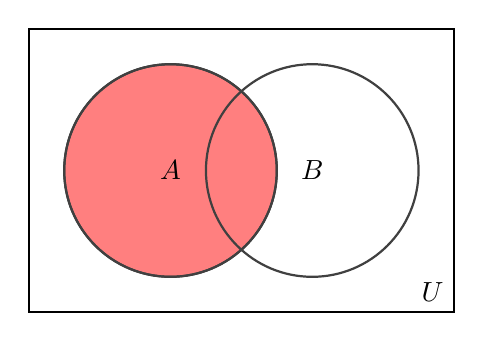
\begin{tikzpicture}[scale=.9]
	\def\circleA{(0,0) circle (1.5)} %A
	\def\circleB{(0:2) circle (1.5)} %B

	\colorlet{circle edgeA}{black!75} 
	\colorlet{circle areaA}{red!100}
	\colorlet{circle edgeB}{black!75} 
	\colorlet{circle areaB}{green!100}

	\tikzset{
		filledA/.style={fill=circle areaA, draw=circle edgeA, thick},
		filledB/.style={fill=circle areaB, draw=circle edgeB, thick},
		outlineA/.style={draw=circle edgeA, thick},
		outlineB/.style={draw=circle edgeB, thick},
	}

	\begin{scope}[fill opacity=0.5]         
			%\fill[filledB] \circleB;    
			\fill[filledA] \circleA;
	\end{scope}

	\draw[outlineA] \circleA node {$A$}; 
	\draw[outlineB] \circleB node {$B$}; 
	%\node[anchor=south] at (current bounding box.north) {$A \cup B$}; 
	\draw[thick] (-2,-2) rectangle (4,2) node[anchor=south east] at (current bounding box.south east) {$U$}; 
\end{tikzpicture} }\only<3-3>{%%%%A or B%%%%%
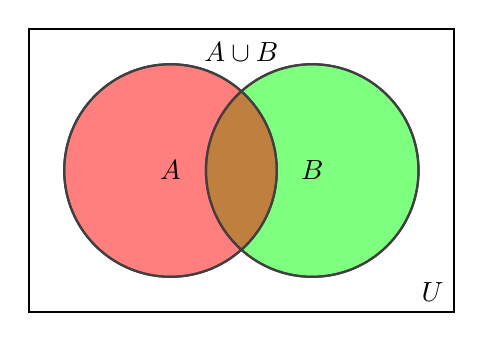
\begin{tikzpicture}[scale=.9]
	\def\circleA{(0,0) circle (1.5)} %A
	\def\circleB{(0:2) circle (1.5)} %B

	\colorlet{circle edgeA}{black!75} 
	\colorlet{circle areaA}{red!100}
	\colorlet{circle edgeB}{black!75} 
	\colorlet{circle areaB}{green!100}

	\tikzset{
		filledA/.style={fill=circle areaA, draw=circle edgeA, thick},
		filledB/.style={fill=circle areaB, draw=circle edgeB, thick},
		outlineA/.style={draw=circle edgeA, thick},
		outlineB/.style={draw=circle edgeB, thick},
	}

	\begin{scope}[fill opacity=0.5]         
			\fill[filledB] \circleB;    
			\fill[filledA] \circleA;
	\end{scope}

	\node[above=-3pt] at (current bounding box.north) {$A \cup B$}; 
	\draw[outlineA] \circleA node {$A$}; 
	\draw[outlineB] \circleB node {$B$}; 
	\draw[thick] (-2,-2) rectangle (4,2) node[anchor=south east] at (current bounding box.south east) {$U$}; 
\end{tikzpicture} }%%%intersection%%%
\only<4-4>{%%%%A colored; B uncolored%%%%%
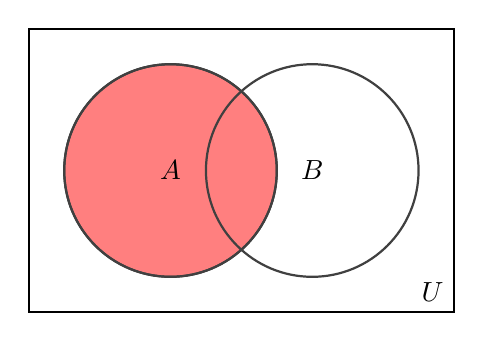
\begin{tikzpicture}[scale=.9]
	\def\circleA{(0,0) circle (1.5)} %A
	\def\circleB{(0:2) circle (1.5)} %B

	\colorlet{circle edgeA}{black!75} 
	\colorlet{circle areaA}{red!100}
	\colorlet{circle edgeB}{black!75} 
	\colorlet{circle areaB}{green!100}

	\tikzset{
		filledA/.style={fill=circle areaA, draw=circle edgeA, thick},
		filledB/.style={fill=circle areaB, draw=circle edgeB, thick},
		outlineA/.style={draw=circle edgeA, thick},
		outlineB/.style={draw=circle edgeB, thick},
	}

	\begin{scope}[fill opacity=0.5]         
			%\fill[filledB] \circleB;    
			\fill[filledA] \circleA;
	\end{scope}

	\draw[outlineA] \circleA node {$A$}; 
	\draw[outlineB] \circleB node {$B$}; 
	%\node[anchor=south] at (current bounding box.north) {$A \cup B$}; 
	\draw[thick] (-2,-2) rectangle (4,2) node[anchor=south east] at (current bounding box.south east) {$U$}; 
\end{tikzpicture} }\only<5-5>{%%%%A or B%%%%%
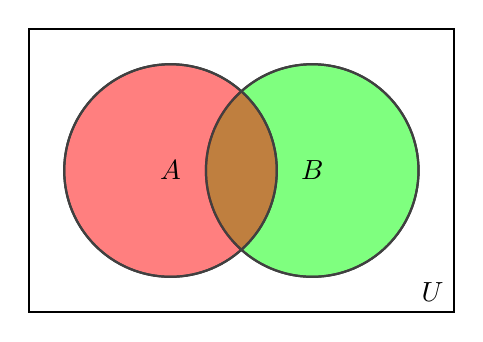
\begin{tikzpicture}[scale=.9]
	\def\circleA{(0,0) circle (1.5)} %A
	\def\circleB{(0:2) circle (1.5)} %B

	\colorlet{circle edgeA}{black!75} 
	\colorlet{circle areaA}{red!100}
	\colorlet{circle edgeB}{black!75} 
	\colorlet{circle areaB}{green!100}

	\tikzset{
		filledA/.style={fill=circle areaA, draw=circle edgeA, thick},
		filledB/.style={fill=circle areaB, draw=circle edgeB, thick},
		outlineA/.style={draw=circle edgeA, thick},
		outlineB/.style={draw=circle edgeB, thick},
	}

	\begin{scope}[fill opacity=0.5]         
			\fill[filledB] \circleB;    
			\fill[filledA] \circleA;
	\end{scope}

	\draw[outlineA] \circleA node {$A$}; 
	\draw[outlineB] \circleB node {$B$}; 
	%\node[anchor=south] at (current bounding box.north) {$A \cup B$}; 
	\draw[thick] (-2,-2) rectangle (4,2) node[anchor=south east] at (current bounding box.south east) {$U$}; 
\end{tikzpicture} }\only<6-6>{%%%%A and B%%%%%
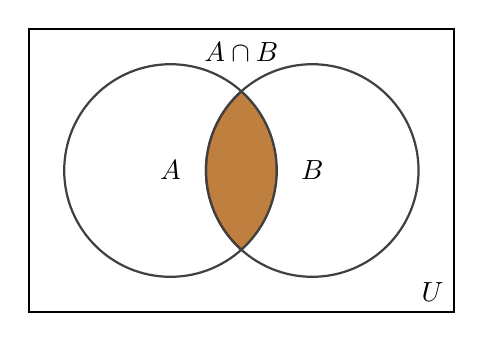
\begin{tikzpicture}[scale=.9]
	\def\circleA{(0,0) circle (1.5)} %A
	\def\circleB{(0:2) circle (1.5)} %B

	\colorlet{circle edgeA}{black!75} 
	\colorlet{circle areaA}{red!100}
	\colorlet{circle edgeB}{black!75} 
	\colorlet{circle areaB}{green!100}

	\tikzset{
		filledA/.style={fill=circle areaA, draw=circle edgeA, thick},
		filledB/.style={fill=circle areaB, draw=circle edgeB, thick},
		outlineA/.style={draw=circle edgeA, thick},
		outlineB/.style={draw=circle edgeB, thick},
	}
	
	\begin{scope}[fill opacity=0.5]    
		\clip \circleA;     
			\fill[filledB] \circleB;
		\clip \circleB;     
			\fill[filledA] \circleA;
	\end{scope}

	\draw[outlineA] \circleA node {$A$}; 
	\draw[outlineB] \circleB node {$B$}; 
	\node[above=-3pt] at (current bounding box.north) {$A \cap B$}; 
	\draw[thick] (-2,-2) rectangle (4,2) node[anchor=south east] at (current bounding box.south east) {$U$}; 
\end{tikzpicture} }\only<7-8>{%%%%A disjoint B%%%%%
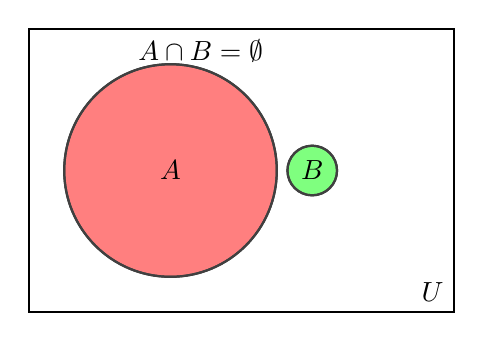
\begin{tikzpicture}[scale=.9]
	\def\circleA{(0,0) circle (1.5)} %A
	\def\circleB{(0:2) circle (.35)} %B

	\colorlet{circle edgeA}{black!75} 
	\colorlet{circle areaA}{red!100}
	\colorlet{circle edgeB}{black!75} 
	\colorlet{circle areaB}{green!100}

	\tikzset{
		filledA/.style={fill=circle areaA, draw=circle edgeA, thick},
		filledB/.style={fill=circle areaB, draw=circle edgeB, thick},
		outlineA/.style={draw=circle edgeA, thick},
		outlineB/.style={draw=circle edgeB, thick},
	}

	\begin{scope}[fill opacity=0.5]         
			\fill[filledB] \circleB;    
			\fill[filledA] \circleA;
	\end{scope}

	\draw[outlineA] \circleA node {$A$}; 
	\draw[outlineB] \circleB node {$B$}; 
	%\node[anchor=south] at (current bounding box.north) {$A \cup B$}; 
	\node[above=-3pt] at (current bounding box.north) {$A \cap B=\emptyset$}; 
	\draw[thick] (-2,-2) rectangle (4,2) node[anchor=south east] at (current bounding box.south east) {$U$}; 
\end{tikzpicture} }%%%complement%%%
\only<9-11>{%%%%A uncolored;%%%%%
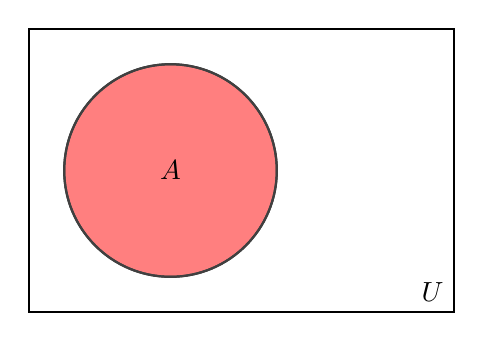
\begin{tikzpicture}[scale=.9]
	\def\circleA{(0,0) circle (1.5)} %A
	\def\circleB{(0:2) circle (1.5)} %B

	\colorlet{circle edgeA}{black!75} 
	\colorlet{circle areaA}{red!100}
	\colorlet{circle edgeB}{black!75} 
	\colorlet{circle areaB}{green!100}

	\tikzset{
		filledA/.style={fill=circle areaA, draw=circle edgeA, thick},
		filledB/.style={fill=circle areaB, draw=circle edgeB, thick},
		outlineA/.style={draw=circle edgeA, thick},
		outlineB/.style={draw=circle edgeB, thick},
	}

	\begin{scope}[fill opacity=0.5]         
			%\fill[filledB] \circleB;    
			\fill[filledA] \circleA;
	\end{scope}

	\draw[outlineA] \circleA node {$A$}; 
	%\draw[outlineB] \circleB node {$B$}; 
	%\node[anchor=south] at (current bounding box.north) {$A \cup B$}; 
	\draw[thick] (-2,-2) rectangle (4,2) node[anchor=south east] at (current bounding box.south east) {$U$}; 
\end{tikzpicture} }\only<12->{%%%%A complement%%%%%
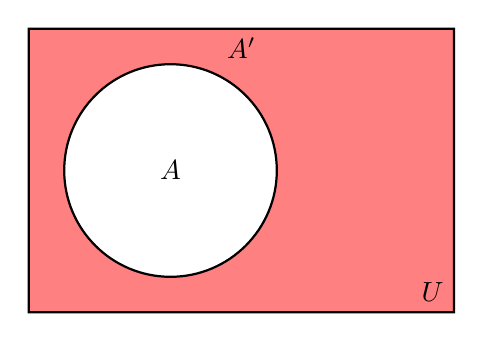
\begin{tikzpicture}[scale=.9]
	\def\circleA{(0,0) circle (1.5)} %A
	\def\circleB{(0:2) circle (1.5)} %B

	\colorlet{circle edgeA}{black!75} 
	\colorlet{circle areaA}{red!100}
	\colorlet{circle edgeB}{black!75} 
	\colorlet{circle areaB}{blue!100}

	\tikzset{
		filledA/.style={fill=circle areaA, draw=circle edgeA, thick},
		filledB/.style={fill=circle areaB, draw=circle edgeB, thick},
		outlineA/.style={draw=circle edgeA, thick},
		outlineB/.style={draw=circle edgeB, thick},
	}

	\draw[thick,fill=red!50,even odd rule] %%even odd rule draws complement of next draw commands%%
		(-2,-2) rectangle (4,2) node[anchor=south east] at (current bounding box.south east) {$U$} 
		\circleA node {$A$};
	\node[below] at (current bounding box.north) {$A'$}; 

\end{tikzpicture} }

\only<8-9>{$A$ and $B$ are \emph{mutually disjoint }if $A\cap B=\emptyset$.}

\only<10->{The \emph{universal set}, denoted $U$, is the set of
all possible elements of any set used in the problem.}
\end{columns}
\end{frame}

\begin{frame}{Set Operations}

\begin{columns}


\column{6cm}

%%%union%%%
\only<1-5>{%%%%A uncolored; B uncolored%%%%%
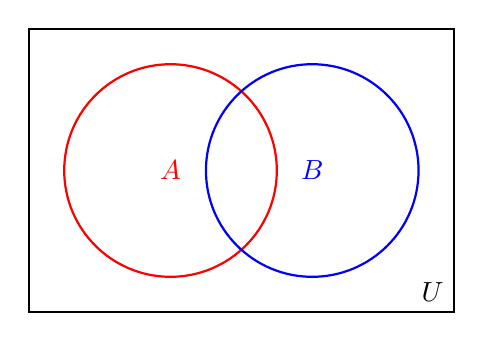
\begin{tikzpicture}[scale=.9]
	\def\circleA{(0,0) circle (1.5)} %A
	\def\circleB{(0:2) circle (1.5)} %B

	\colorlet{circle edgeA}{black!75} 
	\colorlet{circle areaA}{red!100}
	\colorlet{circle edgeB}{black!75} 
	\colorlet{circle areaB}{green!100}

	\tikzset{
		filledA/.style={fill=circle areaA, draw=circle edgeA, thick},
		filledB/.style={fill=circle areaB, draw=circle edgeB, thick},
		outlineA/.style={draw=circle edgeA, thick, red},
		outlineB/.style={draw=circle edgeB, thick, blue},
	}

	\begin{scope}[fill opacity=0.5]         
			%\fill[filledB] \circleB;    
			%\fill[filledA] \circleA;
	\end{scope}

	\draw[outlineA] \circleA node {$A$}; 
	\draw[outlineB] \circleB node {$B$}; 
	%\node[anchor=south] at (current bounding box.north) {$A \cup B$}; 
	\draw[thick] (-2,-2) rectangle (4,2) node[anchor=south east] at (current bounding box.south east) {$U$}; 
\end{tikzpicture} }
\end{columns}
\prob{1}{1}{Let $U=\{M,Tu,W,Th,F,Sa,Su\}$, $A=\{M,Tu,W,Th,F\}$ and $B=\{F,Sa,M\}$. Find the indicated set.}{\center $A\cup B$}

\prob{2}{2}{Let $U$ be the days of the week, $A=\{M,Tu,W,Th,F\}$ and $B=\{F,Sa,M\}$. Find the indicated set.}{\center $A\cap B$}

\prob{3}{3}{Let $U$ be the days of the week, $A=\{M,Tu,W,Th,F\}$ and $B=\{F,Sa,M\}$. Find the indicated set.}{\center $(A\cap B)'$}

\prob{4}{4}{Let $U$ be the days of the week, $A=\{M,Tu,W,Th,F\}$ and $B=\{F,Sa,M\}$. Find the indicated set.}{\center $A' \cup B$}

\prob{5}{5}{Let $U$ be the days of the week, $A=\{M,Tu,W,Th,F\}$ and $B=\{F,Sa,M\}$. Find the indicated set.}{\center $A \cup B'$}
\end{frame}

\begin{frame}{Cardinal Number Formulas}

\vspace{-.5cm}
\begin{columns}


\column{5.5cm}

\ex{1}{}{A researcher collecting data on 100 houses finds that 76 have a DVD player, 21 have a Blue Ray player, and 12 have both.}
\begin{itemize}
\item <1->What is $U$?
\item <2->How many do not have a DVD player?
\item <5->How many have neither a DVD or Blue Ray player?
\item <8->How many have a Blue Ray but not a DVD player?
\end{itemize}

\column{6cm}

%%%blank%%%
\only<1-2>{%%%%A uncolored; B uncolored%%%%%
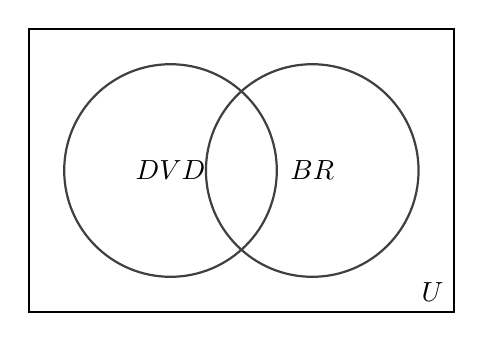
\begin{tikzpicture}[scale=.9]
	\def\circleA{(0,0) circle (1.5)} %A
	\def\circleB{(0:2) circle (1.5)} %B

	\colorlet{circle edgeA}{black!75} 
	\colorlet{circle areaA}{red!100}
	\colorlet{circle edgeB}{black!75} 
	\colorlet{circle areaB}{green!100}

	\tikzset{
		filledA/.style={fill=circle areaA, draw=circle edgeA, thick},
		filledB/.style={fill=circle areaB, draw=circle edgeB, thick},
		outlineA/.style={draw=circle edgeA, thick},
		outlineB/.style={draw=circle edgeB, thick},
	}

	\begin{scope}[fill opacity=0.5]         
			%\fill[filledB] \circleB;    
			%\fill[filledA] \circleA;
	\end{scope}

	\draw[outlineA] \circleA node {$DVD$}; 
	\draw[outlineB] \circleB node {$BR$}; 
	%\node[anchor=south] at (current bounding box.north) {$A \cup B$}; 
	\draw[thick] (-2,-2) rectangle (4,2) node[anchor=south east] at (current bounding box.south east) {$U$}; 
\end{tikzpicture} }\only<3-4>{%%%%A complement%%%%%
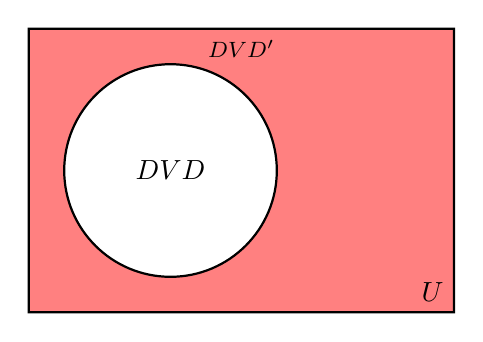
\begin{tikzpicture}[scale=.9]
	\def\circleA{(0,0) circle (1.5)} %A
	\def\circleB{(0:2) circle (1.5)} %B

	\colorlet{circle edgeA}{black!75} 
	\colorlet{circle areaA}{red!100}
	\colorlet{circle edgeB}{black!75} 
	\colorlet{circle areaB}{blue!100}

	\tikzset{
		filledA/.style={fill=circle areaA, draw=circle edgeA, thick},
		filledB/.style={fill=circle areaB, draw=circle edgeB, thick},
		outlineA/.style={draw=circle edgeA, thick},
		outlineB/.style={draw=circle edgeB, thick},
	}

	\draw[thick,fill=red!50,even odd rule] %%even odd rule draws complement of next draw commands%%
		(-2,-2) rectangle (4,2) node[anchor=south east] at (current bounding box.south east) {$U$} 
		\circleA node {$DVD$};
	\node[below=1pt] at (current bounding box.north) {\footnotesize $DVD'$}; 

\end{tikzpicture} }%%%blank%%%
\only<5-5>{%%%%A uncolored; B uncolored%%%%%
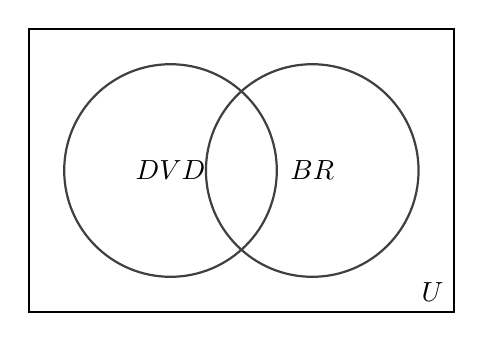
\begin{tikzpicture}[scale=.9]
	\def\circleA{(0,0) circle (1.5)} %A
	\def\circleB{(0:2) circle (1.5)} %B

	\colorlet{circle edgeA}{black!75} 
	\colorlet{circle areaA}{red!100}
	\colorlet{circle edgeB}{black!75} 
	\colorlet{circle areaB}{green!100}

	\tikzset{
		filledA/.style={fill=circle areaA, draw=circle edgeA, thick},
		filledB/.style={fill=circle areaB, draw=circle edgeB, thick},
		outlineA/.style={draw=circle edgeA, thick},
		outlineB/.style={draw=circle edgeB, thick},
	}

	\begin{scope}[fill opacity=0.5]         
			%\fill[filledB] \circleB;    
			%\fill[filledA] \circleA;
	\end{scope}

	\draw[outlineA] \circleA node {$DVD$}; 
	\draw[outlineB] \circleB node {$BR$}; 
	%\node[anchor=south] at (current bounding box.north) {$A \cup B$}; 
	\draw[thick] (-2,-2) rectangle (4,2) node[anchor=south east] at (current bounding box.south east) {$U$}; 
\end{tikzpicture} }\only<6-6>{%%%%A or B%%%%%
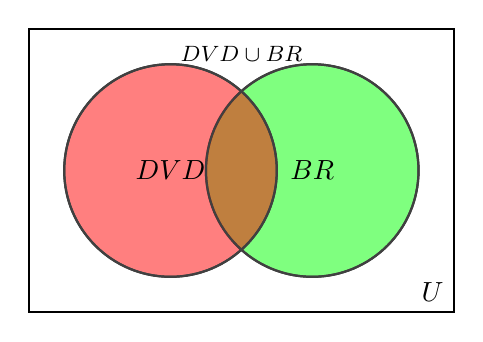
\begin{tikzpicture}[scale=.9]
	\def\circleA{(0,0) circle (1.5)} %A
	\def\circleB{(0:2) circle (1.5)} %B

	\colorlet{circle edgeA}{black!75} 
	\colorlet{circle areaA}{red!100}
	\colorlet{circle edgeB}{black!75} 
	\colorlet{circle areaB}{green!100}

	\tikzset{
		filledA/.style={fill=circle areaA, draw=circle edgeA, thick},
		filledB/.style={fill=circle areaB, draw=circle edgeB, thick},
		outlineA/.style={draw=circle edgeA, thick},
		outlineB/.style={draw=circle edgeB, thick},
	}

	\begin{scope}[fill opacity=0.5]         
			\fill[filledB] \circleB;    
			\fill[filledA] \circleA;
	\end{scope}

	\draw[outlineA] \circleA node {$DVD$}; 
	\draw[outlineB] \circleB node {$BR$}; 
	\node[above=-3pt] at (current bounding box.north) {\footnotesize $DVD \cup BR$}; 
	\draw[thick] (-2,-2) rectangle (4,2) node[anchor=south east] at (current bounding box.south east) {$U$}; 
\end{tikzpicture} }\only<7-7>{%%%%A complement%%%%%
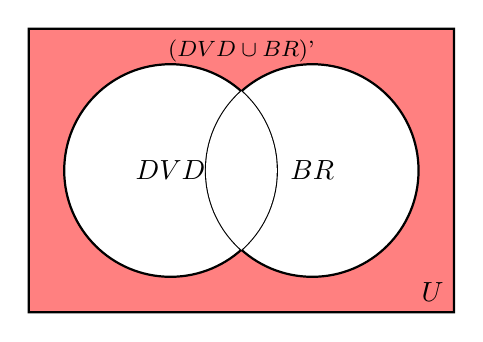
\begin{tikzpicture}[scale=.9]
	\def\circleA{(0,0) circle (1.5)} %A
	\def\circleB{(0:2) circle (1.5)} %B

	\colorlet{circle edgeA}{black!75} 
	\colorlet{circle areaA}{red!100}
	\colorlet{circle edgeB}{black!75} 
	\colorlet{circle areaB}{blue!100}

	\tikzset{
		filledA/.style={fill=circle areaA, draw=circle edgeA, thick},
		filledB/.style={fill=circle areaB, draw=circle edgeB, thick},
		outlineA/.style={draw=circle edgeA, thick},
		outlineB/.style={draw=circle edgeB, thick},
	}

		\draw[thick,fill=red!50,even odd rule] %%even odd rule draws complement of next draw commands%%
			(-2,-2) rectangle (4,2) node[anchor=south east] at (current bounding box.south east) {$U$}
			\circleA node {$DVD$} \circleB node {$BR$};

		\scope 
			\clip (0,0) circle (1.5);%%why can't i use circleA?
			\fill[white] (0:2) circle (1.5); 
		\endscope
		
	\node[below=1pt] at (current bounding box.north) {\footnotesize $(DVD \cup BR$)'}; 

\end{tikzpicture} }%%%blank%%%
\only<8-8>{%%%%A uncolored; B uncolored%%%%%
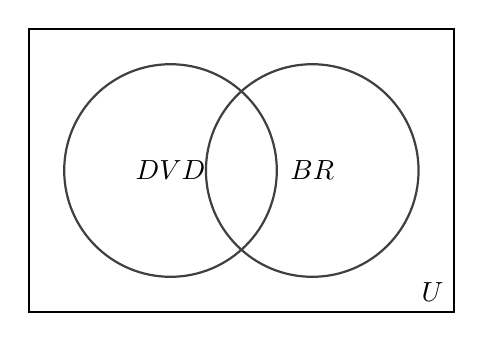
\begin{tikzpicture}[scale=.9]
	\def\circleA{(0,0) circle (1.5)} %A
	\def\circleB{(0:2) circle (1.5)} %B

	\colorlet{circle edgeA}{black!75} 
	\colorlet{circle areaA}{red!100}
	\colorlet{circle edgeB}{black!75} 
	\colorlet{circle areaB}{green!100}

	\tikzset{
		filledA/.style={fill=circle areaA, draw=circle edgeA, thick},
		filledB/.style={fill=circle areaB, draw=circle edgeB, thick},
		outlineA/.style={draw=circle edgeA, thick},
		outlineB/.style={draw=circle edgeB, thick},
	}

	\begin{scope}[fill opacity=0.5]         
			%\fill[filledB] \circleB;    
			%\fill[filledA] \circleA;
	\end{scope}

	\draw[outlineA] \circleA node {$DVD$}; 
	\draw[outlineB] \circleB node {$BR$}; 
	%\node[anchor=south] at (current bounding box.north) {$A \cup B$}; 
	\draw[thick] (-2,-2) rectangle (4,2) node[anchor=south east] at (current bounding box.south east) {$U$}; 
\end{tikzpicture} }\only<9-9>{%%%%A-B%%%%%
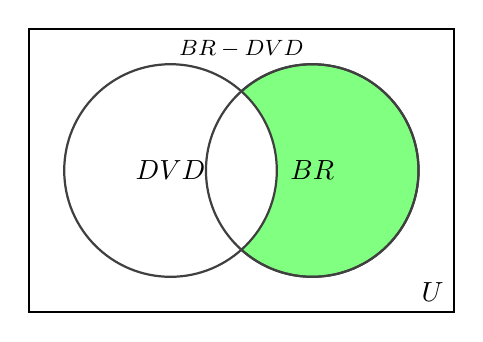
\begin{tikzpicture}[scale=.9]
	\def\circleA{(0,0) circle (1.5)} %A
	\def\circleB{(0:2) circle (1.5)} %B

	\colorlet{circle edgeA}{black!75} 
	\colorlet{circle areaA}{red!50}
	\colorlet{circle edgeB}{black!75} 
	\colorlet{circle areaB}{green!50}

	\tikzset{
		filledA/.style={fill=circle areaA, draw=circle edgeA, thick},
		filledB/.style={fill=circle areaB, draw=circle edgeB, thick},
		outlineA/.style={draw=circle edgeA, thick},
		outlineB/.style={draw=circle edgeB, thick},
	}

	\begin{scope}[shift={(6cm,0cm)}]         
		\begin{scope}[even odd rule]% B-A             
			\clip \circleA (-2,-2) rectangle (4,2);
			\fill[filledB]\circleB;         
		\end{scope}         
		\draw[outlineB] \circleB node {$BR$};         
		\draw[outlineA] \circleA node {$DVD$};
		\draw[thick] (-2,-2) rectangle (4,2) node[anchor=south east] at (current bounding box.south east) {$U$};
	\end{scope}
		
	\node[below=1pt] at (current bounding box.north) {\footnotesize $BR-DVD$}; 

\end{tikzpicture} }

\only<4-4>{
\begin{block}<4-4>{Union Rule}

\begin{itemize}
\item $n(A)+n(A')=n(U)$

\begin{itemize}
\item $n(A)=n(U)-n(A')$
\item $n(A')=n(U)-n(A)$
\end{itemize}
\end{itemize}
\end{block}
}

\begin{block}<5->{Union Rule}

\begin{itemize}
\item $n(A\cup B)=n(A)+n(B)-n(A\cap B)$
\item $n(A\cap B)=n(A\cup B)-n(A)-n(B)$
\end{itemize}
\end{block}
\only<5->{\textbf{Recall: }$n(A)$ is the number of elements in $A$.}
\end{columns}
\end{frame}

\begin{frame}{Problems}

\begin{columns}


\column{6cm}

%%%union%%%
\only<1->{%%%%A uncolored; B uncolored%%%%%
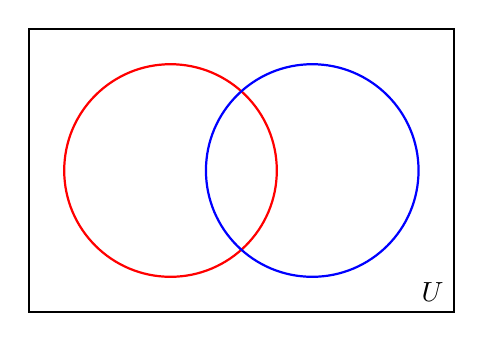
\begin{tikzpicture}[scale=.9]
	\def\circleA{(0,0) circle (1.5)} %A
	\def\circleB{(0:2) circle (1.5)} %B

	\colorlet{circle edgeA}{black!75} 
	\colorlet{circle areaA}{red!100}
	\colorlet{circle edgeB}{black!75} 
	\colorlet{circle areaB}{green!100}

	\tikzset{
		filledA/.style={fill=circle areaA, draw=circle edgeA, thick},
		filledB/.style={fill=circle areaB, draw=circle edgeB, thick},
		outlineA/.style={draw=circle edgeA, thick, red},
		outlineB/.style={draw=circle edgeB, thick, blue},
	}

	\begin{scope}[fill opacity=0.5]         
			%\fill[filledB] \circleB;    
			%\fill[filledA] \circleA;
	\end{scope}

	\draw[outlineA] \circleA node {$$}; 
	\draw[outlineB] \circleB node {$$}; 
	%\node[anchor=south] at (current bounding box.north) {$A \cup B$}; 
	\draw[thick] (-2,-2) rectangle (4,2) node[anchor=south east] at (current bounding box.south east) {$U$}; 
\end{tikzpicture} }
\end{columns}
\prob{1}{1}{Suppose $n(U)=150$, $n(A)=37$, and $n(B)=84$.}{If $n (A\cup B)=100$ find $n(A\cap B)$ and shade in the Venn to represent the indicated set.}

\prob{2}{2}{Suppose $n(U)=150$, $n(A)=37$, and $n(B)=84$.}{If $n (A\cup B)=121$ find $n(A\cap B)$ and shade in the Venn to represent the indicated set.}

\prob{3}{3}{In a recent survey of $500$ high school senior, it was found that $102$ owned an automobile, $147$ owned a motorcycle, and $21$ owned both.}{Draw a Venn diagram illustrating the results of the survey.}

\prob{4}{4}{In a recent survey of $500$ high school senior, it was found that $102$ owned an automobile, $147$ owned a motorcycle, and $21$ owned both.}{What percent of these students own an automobile or a motorcycle.}

\prob{5}{5}{In a recent survey of $500$ high school senior, it was found that $102$ owned an automobile, $147$ owned a motorcycle, and $21$ owned both.}{What percent of these students own an automobile and a motorcycle.}

\prob{6}{6}{Determine how many cards, in an ordinary deck of playing cards, fit the description.}{Spades or aces.}

\prob{7}{7}{Determine how many cards, in an ordinary deck of playing cards, fit the description.}{Face cards and red.}

\prob{8}{8}{Determine how many cards, in an ordinary deck of playing cards, fit the description.}{Face cards and red.}

\prob{9}{9}{Answer the following.}{If $A\cap B= \emptyset$, what is the relationshiop between $A$ and $B$.}

\prob{10}{10}{Answer the following.}{If $A\cup B= \emptyset$, what is the relationshiop between $A$ and $B$.}

\prob{11}{11}{Answer the following.}{If  $A\cap B= B$, what must be true concerning these two sets.}

\prob{12}{12}{Answer the following.}{If  $A\cup B= B$, what must be true concerning these two sets.}

\prob{13}{13}{Answer the following.}{If  $A\cap A= \emptyset$, what must be true concerning $A$.}
\end{frame}

\end{document}
